%%%%%%%%%%%%%%%%%%%%%%%%%%%%%%%%%%%%%%%%%
% baposter Landscape Poster
% LaTeX Template
% Version 1.0 (11/06/13)
%
% baposter Class Created by:
% Brian Amberg (baposter@brian-amberg.de)
%
% This template has been downloaded from:
% http://www.LaTeXTemplates.com
%
% License:
% CC BY-NC-SA 3.0 (http://creativecommons.org/licenses/by-nc-sa/3.0/)
%
%%%%%%%%%%%%%%%%%%%%%%%%%%%%%%%%%%%%%%%%%

%----------------------------------------------------------------------------------------
%	PACKAGES AND OTHER DOCUMENT CONFIGURATIONS
%----------------------------------------------------------------------------------------

\documentclass[portrait,a0paper,fontscale=0.285]{baposter} % Adjust the font scale/size here

\frenchspacing

\usepackage{braket}     %required for quantum
\usepackage{amsmath}    %required for quantum
\usepackage{mathtools}  %required for quantum
\usepackage{nccmath}    %required for quantum
\usepackage{wrapfig}    %required for quantum
\usepackage{hyperref}
 
\usepackage{graphicx} % Required for including images
\graphicspath{{figures/}} % Directory in which figures are stored

\usepackage{amsmath} % For typesetting math
\usepackage{amssymb} % Adds new symbols to be used in math mode

\usepackage{booktabs} % Top and bottom rules for tables
\usepackage{enumitem} % Used to reduce itemize/enumerate spacing
\usepackage{palatino} % Use the Palatino font
\usepackage[font=small,labelfont=bf]{caption} % Required for specifying captions to tables and figures

\usepackage{multicol} % Required for multiple columns
\setlength{\columnsep}{1.5em} % Slightly increase the space between columns
\setlength{\columnseprule}{0mm} % No horizontal rule between columns

\usepackage{tikz} % Required for flow chart
\usetikzlibrary{shapes,arrows} % Tikz libraries required for the flow chart in the template

\usepackage{epstopdf}

\newcommand{\compresslist}{ % Define a command to reduce spacing within itemize/enumerate environments, this is used right after \begin{itemize} or \begin{enumerate}
\setlength{\itemsep}{1pt}
\setlength{\parskip}{0pt}
\setlength{\parsep}{0pt}
}

\definecolor{lightblue}{rgb}{0.145,0.6666,1} % Defines the color used for content box headers

\definecolor{ourred}{rgb}{0.9,0.0,0.0}

\begin{document}

\begin{poster}
{
headerborder=closed, % Adds a border around the header of content boxes
colspacing=1em, % Column spacing
bgColorOne=white, % Background color for the gradient on the left side of the poster
bgColorTwo=white, % Background color for the gradient on the right side of the poster
borderColor=lightblue, % Border color
headerColorOne=black, % Background color for the header in the content boxes (left side)
headerColorTwo=lightblue, % Background color for the header in the content boxes (right side)
headerFontColor=white, % Text color for the header text in the content boxes
boxColorOne=white, % Background color of the content boxes
textborder=roundedleft, % Format of the border around content boxes, can be: none, bars, coils, triangles, rectangle, rounded, roundedsmall, roundedright or faded
eyecatcher=true, % Set to false for ignoring the left logo in the title and move the title left
headerheight=0.1\textheight, % Height of the header
headershape=roundedright, % Specify the rounded corner in the content box headers, can be: rectangle, small-rounded, roundedright, roundedleft or rounded
headerfont=\Large\bf\textsc, % Large, bold and sans serif font in the headers of content boxes
%textfont={\setlength{\parindent}{1.5em}}, % Uncomment for paragraph indentation
linewidth=2pt % Width of the border lines around content boxes
}
%----------------------------------------------------------------------------------------
%	TITLE SECTION 
%----------------------------------------------------------------------------------------
%
{
\includegraphics[height=8.6em]{leidenland.pdf}} % First university/lab logo on the left
{\bf\textsc{\textcolor{ourred}{The effects of noise on quantum algorithms solving 3SAT}}\vspace{-0.1em}} % Poster title
{\textsc{\begin{large}Martijn Swenne\end{large} \begin{small}(supervized by Vedran Dunjko)\end{small}\\ \begin{small}Leiden Institute of Advanced Computer Science\end{small}\\[0.5mm]}\begin{footnotesize}\texttt{s1923889@liacs.leidenuniv.nl}\end{footnotesize}} % Author names and institution

%----------------------------------------------------------------------------------------
%	OVERVIEW
%----------------------------------------------------------------------------------------

\headerbox{Overview}{name=overview,column=0,row=0}{

\textcolor{ourred}{\textsc{Quantum}} is a term you hear a lot lately. Quantum computing uses quantum-mechanical phenomena, such as superposition and entanglement. A quantum computer is therefor completely different than a classical computer. Whereas a classical computer uses binary digits, which are always in one of two definite states (0 or 1), a quantum computer uses quantum bits, or \textcolor{ourred}{\textsc{qubits}}. These qubits can be in a superposition of states. Quantum computers are extremely powerful, but also very noisy. This is currently a big problem in quantum computers.

}

%----------------------------------------------------------------------------------------
%	Basics
%----------------------------------------------------------------------------------------

\headerbox{Basics}{name=basics,column=0,below=overview}{ % This block's bottom aligns with the bottom of the conclusion block

A \textcolor{ourred}{\textsc{quantum computer}} operates on qubits using quantum gates and measurement. It maintains a sequence of $n$ qubits, which can represent a $0$, a $1$ or any quantum superposition of those two states. Measurements collapse the system of qubits into one of the $2^{n}$ states, decomposing into a classical state. Quantum algorithms are often probabilistic. They provide the correct solution only with a certain known probability. 


Qubits are represented in the \textcolor{ourred}{\textsc{Dirac}} notation. There is the ket $\ket{0}$ and the hermitan conjugate called the bra $\bra{0}$. Qubits and quantum gates can be described with matrices. For instance:

$\ket{0} = 
\begin{bsmallmatrix}
	1 \\
	0 \\
\end{bsmallmatrix}$
\hfill and \hfill 
$\ket{1} = 
\begin{bsmallmatrix}
	0 \\
	1 \\
\end{bsmallmatrix}$

Just as in classical computations, where you work with classical logic gates, quantum computations work with quantum logic gates, which are 1 or 2 qubit gates. Unlike classical logic gates, these gates are reversible. For instance, a basic quantum logic gate is the Hadamard gate:

\begin{center}
		$H\ket{0} = \frac{1}{\sqrt{2}}
		\begin{bsmallmatrix}
			1 & 1 \\
			1 & $-$1 \\
		\end{bsmallmatrix}
		\begin{bsmallmatrix}
			1 \\
			0 \\
		\end{bsmallmatrix}
		=	\frac{1}{\sqrt{2}}
		\begin{bsmallmatrix}
			1 \\
			1 \\
		\end{bsmallmatrix}
		=
		\frac{\ket{0}+\ket{1}}{\sqrt{2}}$	
	
		$H\ket{1} = \frac{1}{\sqrt{2}}
		\begin{bsmallmatrix}
			1 & 1 \\
			1 & $-$1 \\
		\end{bsmallmatrix}
		\begin{bsmallmatrix}
			0 \\
			1 \\
		\end{bsmallmatrix}
		=	\frac{1}{\sqrt{2}}
		\begin{bsmallmatrix}
			1 \\
			$-$1 \\
		\end{bsmallmatrix}
		=
		\frac{\ket{0}-\ket{1}}{\sqrt{2}}$
\end{center}

The Hadamard gate puts the qubit in a superposition of basis states. The probability that the qubit is $\ket{0}$ is $(\frac{1}{\sqrt{2}})^{2}=0.5$. The probability for $\ket{1}$ is also $0.5$. There is another basic quantum gate, which is called the CNOT-gate. This is a controlled-NOT gate. The gate flips the state of the target qubit if and only if the control qubit is $1$.

\begin{center}

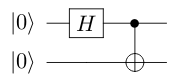
\includegraphics[scale=0.7]{H_CNOT_circuit.png}

\end{center}

If you now apply a Hadamard gate on the control qubit before a CNOT-gate, the two qubits become \textcolor{ourred}{\textsc{entangled}}. This means that you cannot describe a qubit independently of the state of the other qubit. If you were to measure the state of the first qubit, it immediately tells you the state of the second qubit, because thats our only possibility. This representation is called a Bell-state, which is a maximally entangled state.

}

%----------------------------------------------------------------------------------------
%	Solving 3SAT
%----------------------------------------------------------------------------------------

\headerbox{Solving 3-SAT}{name=solvingSAT,column=2,row=0}{

The \textcolor{ourred}{\textsc{boolean satisfiability}} problem is the problem of determining if there exists an interpretation that satisfies a given Boolean formula. SAT is proven to be NP-complete. This means that it is solvable in polynomial time.

A special case of boolean satisfiability is the \textcolor{ourred}{\textsc{3-SAT}}. This means the boolean formula is in conjunctive normal form where each clause is limited to at most three literals. Each clause has to be satisfied, while in every clause only one out of the three literals has to be satisfied. Such a boolean formula can be written like:

\vspace{-0.5em}
\begin{center}
$(l_{1} \lor l_{2} \lor l_{3}) \land \dots \land (l_{1} \lor l_{2} \lor l_{3})$
\end{center}
\vspace{-0.5em}

For the 3-SAT there exists a quantum algorithm that solves it brute force in $O(2^{n/2})$, while a classical brute force solves it in $O(2^{n})$. This quantum algorithm is called \textcolor{ourred}{\textsc{Grover's search}}.

\vspace{-0.5em}
\begin{center}
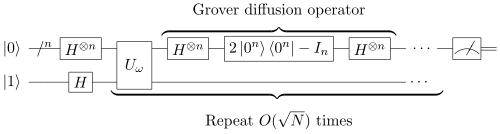
\includegraphics[scale=0.4]{Grovers_algorithm.png}

\begin{tiny}Wikipedia; Grover's algorithm\end{tiny}
\end{center}
\vspace{-0.5em}


Although this is significantly better than a classical brute force, the best classical algorithm for 3-SAT, the \textcolor{ourred}{\textsc{Sch\"{o}ning}} algorithm (walkSAT), solves it in $O(\frac{4}{3}^{n})=O(2^{0.415*n})$. This means that a brute force quantum algorithm is still slower than the fastest classical algorithm. 

}

%----------------------------------------------------------------------------------------
%	Image
%----------------------------------------------------------------------------------------

\headerbox{Quantum computer}{name=Image,column=1,row=0, bottomaligned=solvingSAT}{

The image below is a quantum computer from IBM.

\begin{center}
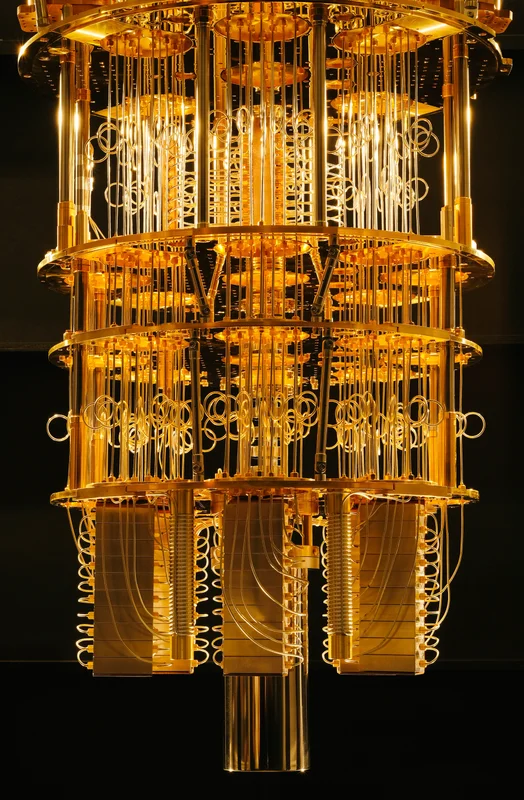
\includegraphics[scale=0.25]{quantum_computer.png}

\begin{tiny}IBM Research Flickr (2018)\end{tiny}
\end{center}
Below is an example of code to implement a quantum circuit. This is a python library called \textcolor{ourred}{\textsc{Qiskit}}.
\begin{center}
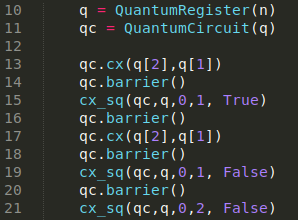
\includegraphics[scale=0.35]{Code.png}
\end{center}

}

\headerbox{PromiseBall}{name=promiseball,column=1,below=solvingSAT, bottomaligned=basics}{

The \textcolor{ourred}{\textsc{PromiseBallSAT}} (or PBS) is a derandomized Sch\"{o}ning algorithm for a ($\leq$k)-CNF formula. Given the randomized initial assignment $x$, let $B_{r}(x)$ denote the $r$-ball centered at $x$, i.e. the set of all bitstrings $y$ has a \textcolor{ourred}{\textsc{Hamming distance}} $\leq r$. The space of possible assignments is covered by a number of $r$-balls.

\begin{center}
	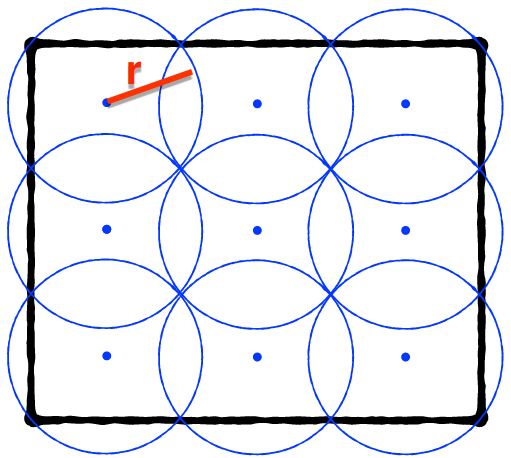
\includegraphics[scale=0.18]{PromiseBall.png}

	\begin{tiny}Vedran Dunjko (2018)\end{tiny}
\end{center}
Given such a covering set, specified by the centers of the balls, the algorithm sequentially checks whether there exists a satisfying assignment within each of the r-balls. The deterministic algorithm $PromiseBall(F,r,x)$ is a simple, recursive divide-and-conquer algorithm. It first checks some obvious conditions for (un)satisfiability, or if $x$ is a satisfying assignment. Otherwise, in the recursive step, it finds the first unsatisfied clause $C$, and calls $Promise-Ball(F^{[l=1]},r−1,x)$ for every literal $l\in C$. Here,$F^{[l=1]}$ denotes the formula obtained by setting the variable corresponding to $l$ to the value ensuring $l=1$,i.e., all clauses involving $l$ are removed (or truncated).
	
}

%----------------------------------------------------------------------------------------
%	Quantum noise
%----------------------------------------------------------------------------------------

\headerbox{Quantum noise}{name=noise,column=2,below=solvingSAT}{

\textcolor{ourred}{\textsc{Quantum decoherence}}, or quantum noise, happens when qubits lose information to the environment over time. This doesn't start until the qubits are used, like measuring them or performing a computation. 

There's a certain threshold for noise, which is called \textcolor{ourred}{\textsc{fault tolerance}}, where quantum computers will theoretically be reliable enough to be considered useful. Up to this moment, there is no good solution to this problem. Quantum noise currently gets simulated by adding random gates (such as the Pauli X gate) into the circuit.

}


%----------------------------------------------------------------------------------------
%	FURTHER RESEARCH
%----------------------------------------------------------------------------------------

\headerbox{Further research}{name=further,column=2,below=noise,bottomaligned=basics}{

\begin{enumerate}[label= {[\arabic*]}]
	\item A full derandomization of sch\"{o}ning's k-SAT algorithm; https://dl.acm.org/ci-tation.cfm?doid=1993636.1993670
	\item Quantum Computing in the NISQ era and beyond; https://arxiv.org/ abs/1801.00862
	\item 3-SAT Faster and Simpler - Unique-SAT Bounds for PPSZ Hold in General; https://epubs.siam.org/doi/10.1137/1 20868177
	\item Computational speedup using small quantum devices; https://arxiv.org/ pdf/1807.08970.pdf
\end{enumerate}
}

%----------------------------------------------------------------------------------------

\end{poster}

\end{document}
